\documentclass[aspectratio=169,xcolor=dvipsnames]{beamer}

\usepackage{amsthm}
\usepackage{amsmath}
\usepackage{amssymb}
\usepackage{tikz}
\usepackage{pgfplots}
\usepackage{xfp}
\pgfplotsset{compat=1.18}
\usepackage[authoryear, round]{natbib}
\usepackage{hyperref}
\usetikzlibrary{arrows.meta,positioning,decorations.pathreplacing}
\hypersetup{
    colorlinks=true,
    linkcolor=blue,
    citecolor=blue,
    urlcolor=blue
}

\definecolor{darkgreen}{rgb}{0,0.5,0}
\definecolor{darkblue}{rgb}{0,0,0.55}

\newtheorem{proposition}{Proposition}
\setbeamertemplate{footline}[frame number]
\usetheme{Frankfurt}
\usefonttheme{serif}

% Title info
\title{Extreme Value Theory with Heterogeneous Agents}
\subtitle{\normalsize Sephorah Mangin (2025)}
\author{Presented by Simon Mishricky}
\institute{TV$=$V Reading Group \\ Research School of Economics, Australian National University}
\date{\today}

\begin{document}
\section{Motivation}
\frame{\titlepage}

\begin{frame}{Where extreme outcomes show up}
    Many objects of economic interest are determined by a \emph{maximum} (or a minimum):
    \begin{itemize}
        \item firm productivity $=$ best idea drawn from $G$;
        \item consumer surplus $=$ best of $n$ price quotes;
        \item OTC execution price $=$ best of $k$ broker quotes \hfill {\small (Mishricky 2026)};
        \item peer outcome $=$ most studious friend;
        \item top income, longest spell, largest shock, $\ldots$
    \end{itemize}
    \vspace{3mm}
    Classical theory (Fisher--Tippett--Gnedenko) tells us:
    \begin{itemize}
        \item if $X_1,\dots,X_n \overset{iid}{\sim} G$, the normalised max converges to one of
        \item \textbf{three} extreme value distributions: Fr\'echet, Gumbel, Weibull.
    \end{itemize}
\end{frame}

\begin{frame}{The question}
    Classical EV theory assumes every agent receives the \textbf{same} number of draws $n$.
    \vspace{3mm}

    But in many economic settings, this number is itself random and varies across agents:
    \begin{itemize}
        \item firms differ in R\&D intensity $\Rightarrow$ different numbers of ideas;
        \item consumers differ in attention $\Rightarrow$ different numbers of price quotes;
        \item students differ in popularity $\Rightarrow$ different numbers of friends.
    \end{itemize}
    \vspace{3mm}
    \textbf{Question.} What does the EV theory look like when the number of draws is itself a random variable, drawn from a distribution that captures heterogeneity across agents?
\end{frame}

\begin{frame}{Takeaways}
    \begin{enumerate}
        \item A clean, tractable generalisation of EV theory in which the number of draws is mixed Poisson.
        \vspace{2mm}
        \item The three classical EV distributions arise only in a knife-edge case (Poisson).
        \vspace{2mm}
        \item Heterogeneity in draws shows up in extreme outcomes through a single correction factor $\mathbb{E}_F[X^{-\rho}]$.
        \vspace{2mm}
        \item Mean-preserving spreads in heterogeneity can \emph{increase or decrease} extreme outcomes -- the sign is pinned down by the tail index $\gamma$.
    \end{enumerate}
\end{frame}

\section{Setup}
\begin{frame}{A warm-up derivation: Pareto $\to$ Fr\'echet}
    Let $X_1,\dots,X_n \overset{iid}{\sim} \text{Pareto}$: $G(x) = 1 - x^{-1/\gamma}$ for $x\ge 1$, $\gamma>0$.

    \vspace{2mm}
    Pick the normalisation $a_n = n^\gamma$ and study $Z_n \equiv M_n / n^\gamma$:
    \begin{align*}
        \Pr(Z_n \le x)
        \;&=\; \Pr(M_n \le n^\gamma x)
        \;=\; G(n^\gamma x)^n
        \;=\; \left(1 - (n^\gamma x)^{-1/\gamma}\right)^n \\[1mm]
        \;&=\; \left(1 - \tfrac{x^{-1/\gamma}}{n}\right)^n
        \;\xrightarrow{n\to\infty}\; e^{-x^{-1/\gamma}}.
    \end{align*}
    \vspace{1mm}

    That's the \textbf{Fr\'echet} distribution. The whole engine is the identity $(1-u/n)^n \to e^{-u}$ applied to the tail $1-G$.

    \vspace{2mm}
    Generalising the tail behaviour of $G$ from Pareto to ``tail index $\gamma$'' gives the three classical EV types.
\end{frame}

\begin{frame}{Classical EV theory: fixed number of draws}
    Let $X_1,\dots,X_n \overset{iid}{\sim} G$ with tail index $\gamma\in\mathbb{R}$:
    \[
        \gamma \;\equiv\; \lim_{x\to\overline{x}} \frac{d}{dx}\!\left(\frac{1-G(x)}{g(x)}\right).
    \]
    Define $M_n \equiv \max\{X_1,\dots,X_n\}$. Then $\Pr(M_n\le x)=G(x)^n$.

    \vspace{2mm}
    \textbf{Fisher--Tippett--Gnedenko.} There exist constants $a_n, b_n$ such that $Z_n \equiv a_n M_n + b_n$ converges in distribution to
    \[
        H_\gamma(x) \;=\; e^{-v_\gamma(x)},\qquad
        v_\gamma(x) \;=\;
        \begin{cases}
            (1+\gamma x)^{-1/\gamma}, & \gamma\ne 0,\\
            e^{-x}, & \gamma=0.
        \end{cases}
    \]
    \begin{itemize}
        \item $\gamma>0$: \textbf{Fr\'echet} (fat tails, e.g.\ Pareto);
        \item $\gamma=0$: \textbf{Gumbel} (thin tails, e.g.\ exponential);
        \item $\gamma<0$: \textbf{reverse-Weibull} (bounded support).
    \end{itemize}
\end{frame}

\begin{frame}{Random number of draws}
    Replace $n$ with a random variable $N(\theta)\in\mathbb{N}$ with mean $\theta$:
    \[
        M_{N(\theta)} \;\equiv\; \max\{X_1,\dots,X_{N(\theta)}\}.
    \]
    \vspace{1mm}

    Two interpretations of the distribution $P_n(\theta) \equiv \Pr(N(\theta)=n)$:
    \begin{itemize}
        \item \emph{Within-agent randomness:} a given agent's draw count is noisy.
        \item \emph{Cross-agent heterogeneity:} different agents are different \textbf{types}, and types differ in their expected number of draws.
    \end{itemize}

    \vspace{3mm}
    We take the limit $\theta\to\infty$ (a ``large economy'').

    \vspace{2mm}
    \textbf{Question.} Does the limiting distribution of the (normalised) max still satisfy the FTG trichotomy?
\end{frame}

\begin{frame}{The mixed Poisson class}
    \textbf{Assumption.} $N(\theta)$ is mixed Poisson:
    \[
        N(\theta)\,\big|\,\tau \;\sim\; \mathrm{Poisson}(\theta\tau),\qquad \tau\sim F,\qquad \mathbb{E}_F[\tau]=1.
    \]
    Here $\tau$ is the agent's \textbf{type} and $F$ is the type distribution.

    \vspace{3mm}
    Choosing $F$ recovers familiar discrete distributions:
    \begin{center}
        \begin{tabular}{ll}
            $F = \delta_1$ & Poisson \\
            $F = \Gamma(r,r)$ & negative binomial \\
            $F = \text{Exp}(1)$ & geometric \\
            $F = $ Pareto & power-law
        \end{tabular}
    \end{center}
\end{frame}

\begin{frame}{The key sufficient statistic: $P_0$}
    The probability of \emph{zero} draws is everything we need.
    Define
    \[
        P_0(\theta) \;\equiv\; \Pr(N(\theta)=0) \;=\; \int_0^\infty e^{-\theta\tau}\,dF(\tau),
    \]
    the Laplace transform of the type distribution $F$.

    \vspace{3mm}
    \begin{lemma}
        $\;\;H_P(x;\theta) \;\equiv\; \Pr(M_{N(\theta)}\le x) \;=\; P_0\!\left(\theta\,(1-G(x))\right).$
    \end{lemma}

    \vspace{3mm}
    \emph{Sketch.} The pgf of $N(\theta)$ is $\mathbb{E}[y^{N(\theta)}] = P_0(\theta(1-y))$; set $y=G(x)$.
\end{frame}

\begin{frame}{Asymptotic dispersion}
    Measure dispersion by the squared coefficient of variation:
    \[
        cv^2_P(\theta) \;=\; \frac{1}{\theta} + cv^2_F
        \quad\xrightarrow{\theta\to\infty}\quad
        cv^2_F.
    \]
    \begin{itemize}
        \item Poisson noise ($1/\theta$) washes out in the large-$\theta$ limit.
        \item The \textbf{residual} dispersion is $cv^2_F$ -- the heterogeneity of types.
    \end{itemize}
    \vspace{3mm}

    \textbf{Punchline.} A naive LLN argument would suggest heterogeneity disappears in the limit. It doesn't: $cv^2_F$ survives, and it drives everything that follows.
\end{frame}

\section{The extreme value distribution}

\begin{frame}{Main result: a new class of EV distributions}
    \begin{theorem}[Mangin, 2025]
        Let $G$ have tail index $\gamma\in\mathbb{R}$ and let $P_n$ be mixed Poisson with type distribution $F$. Then there exist constants $a_\theta, b_\theta$ such that $Z_{N(\theta)} \equiv a_\theta M_{N(\theta)} + b_\theta$ converges in distribution as $\theta\to\infty$ to
        \[
            \boxed{\;H_{\gamma,P}(x) \;=\; P_0\!\left(v_\gamma(x)\right)\;}
        \]
        where $v_\gamma(x) = (1+\gamma x)^{-1/\gamma}$ for $\gamma\ne 0$ and $v_\gamma(x)=e^{-x}$ for $\gamma=0$.
    \end{theorem}
    \vspace{2mm}
    Two pieces of data determine the limiting distribution:
    \begin{itemize}
        \item the \textbf{tail index} $\gamma$ of $G$;
        \item the \textbf{Laplace transform} $P_0$ of the type distribution $F$.
    \end{itemize}
    Classical FTG recovered when $F$ is degenerate: $P_0(z)=e^{-z}$, so $H_{\gamma,P}=H_\gamma$.
\end{frame}

\begin{frame}{Sketch of Theorem 1}
    Condition on the type $\tau$. Then $N(\theta)\,|\,\tau \sim \text{Poisson}(\theta\tau)$, which is essentially $\theta\tau$ deterministic draws as $\theta\to\infty$. Classical EV theory gives
    \[
        \Pr(Z_{N(\theta)} \le x \,|\, \tau) \;\longrightarrow\; H_\gamma(x)^\tau.
    \]
    Averaging over $\tau\sim F$:
    \[
        H_{\gamma,P}(x) \;=\; \int_0^\infty H_\gamma(x)^\tau\, dF(\tau) \;=\; P_0(v_\gamma(x)),
    \]
    using $H_\gamma(x) = e^{-v_\gamma(x)}$ and the definition of $P_0$. \qed

    \vspace{3mm}
    \footnotesize Formally: Barndorff-Nielsen (1964) does the conditioning step, and $N(\theta)/\theta \xrightarrow{p} \tau$ (Chebyshev on the conditional Poisson) does the averaging step.
\end{frame}

\begin{frame}{Heterogeneity is a drag on the maximum}
    \begin{corollary}[First-order stochastic dominance]
        If $P_n$ is mixed Poisson but not Poisson, then $H_\gamma$ first-order stochastically dominates $H_{\gamma,P}$:
        $\;H_{\gamma,P}(x) > H_\gamma(x)$ for all $x$.
    \end{corollary}
    \vspace{2mm}
    \emph{Why?} $\;\tau\mapsto z^\tau$ is convex for $z\in(0,1)$, so Jensen gives
    \[
        H_{\gamma,P}(x) \;=\; \mathbb{E}_F[H_\gamma(x)^\tau] \;>\; H_\gamma(x)^{\mathbb{E}_F[\tau]} \;=\; H_\gamma(x).
    \]

    \vspace{2mm}
    \textbf{Intuition.} Diminishing returns to draws. Spreading draws unequally across agents lowers the expected maximum -- heterogeneity is misallocation.
\end{frame}

\begin{frame}{Poisson is the knife-edge case}
    \begin{corollary}[Uniqueness of Poisson]
        $H_{\gamma,P} = H_\gamma$ if and only if $P_n$ is Poisson.
    \end{corollary}
    \vspace{2mm}

    The three classical EV types (Fr\'echet, Gumbel, Weibull) arise \emph{only} when $F$ is degenerate.

    \vspace{2mm}
    Once we admit any heterogeneity in types, the limiting distribution leaves the FTG trichotomy and lands in a larger class $\{H_{\gamma,P}\}$ indexed by $(\gamma, F)$.

    \vspace{3mm}
    \textbf{Two further properties of this class.}
    \begin{itemize}
        \item \emph{Max-stability.} If $G = H_{\gamma,P}$, then applying the same mixed-Poisson EV operator returns $H_{\gamma,P}$. (Generalises stability of the three classical types.)
        \item \emph{Tail inheritance.} $H_{\gamma,P}$ has tail index $\gamma$. Heterogeneity affects the body, not the tail.
    \end{itemize}
\end{frame}

\begin{frame}{Picture: negative binomial family ($G$ Pareto, $\gamma=1/2$)}
    \centering
    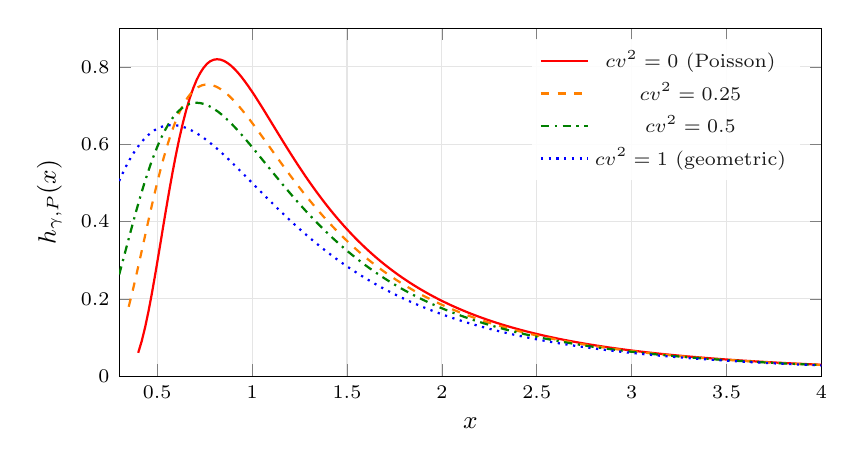
\begin{tikzpicture}
        \begin{axis}[
            width=10.5cm, height=6cm,
            xlabel={$x$}, ylabel={$h_{\gamma,P}(x)$},
            xmin=0.3, xmax=4, ymin=0, ymax=0.9,
            legend pos=north east,
            legend style={font=\scriptsize, fill=white, fill opacity=0.9, draw=none},
            tick label style={font=\scriptsize},
            label style={font=\small},
            grid=both, grid style={gray!20}
        ]
        % cv^2 = 0 (Poisson) -> Frechet density
        \addplot[red, thick, samples=200, domain=0.4:4] {2*x^(-3) * exp(-x^(-2))};
        \addlegendentry{$cv^2=0$ (Poisson)}
        % cv^2 = 0.25 (r=4): h = 2 x^{-3} (r/(r+x^{-2}))^{r+1}
        \addplot[orange, thick, dashed, samples=200, domain=0.35:4]
            {2*x^(-3)*(4/(4+x^(-2)))^5};
        \addlegendentry{$cv^2=0.25$}
        % cv^2 = 0.5 (r=2): h = 2 x^{-3} (r/(r+x^{-2}))^{r+1}
        \addplot[darkgreen, thick, dashdotted, samples=200, domain=0.3:4]
            {2*x^(-3)*(2/(2+x^(-2)))^3};
        \addlegendentry{$cv^2=0.5$}
        % cv^2 = 1 (geometric, r=1)
        \addplot[blue, thick, dotted, samples=200, domain=0.3:4]
            {2*x^(-3)*(1/(1+x^(-2)))^2};
        \addlegendentry{$cv^2=1$ (geometric)}
        \end{axis}
    \end{tikzpicture}\\
    \footnotesize Greater dispersion $cv^2_F$ shifts mass leftward (FOSD) but preserves the Fr\'echet tail index $\gamma=1/2$.
\end{frame}

\section{Extreme value outcomes}

\begin{frame}{From distribution to outcomes}
    Economic models care about expectations of \emph{functions} of the max:
    \[
        \mathbb{E}\bigl[\zeta(M_{N(\theta)})\bigr],\qquad \zeta:[\underline{x},\overline{x}]\to\mathbb{R}_+.
    \]
    Examples:
    \begin{itemize}
        \item aggregate productivity: $\zeta(x) = x$;
        \item expected markup: $\zeta(x) = (1-G(x))/g(x)$ (Mills ratio).
    \end{itemize}
    \vspace{2mm}
    \textbf{Regular variation.} Assume $\zeta(G^{-1}(1-t)) \sim t^\rho$ as $t\to 0$, for some $\rho>-1$. The index $\rho$ summarises how $\zeta$ scales near the upper tail of $G$.

    \vspace{2mm}
    For $\zeta(x)=x$ and unbounded support: $\rho = -\gamma$ (the tail index of $G$).
\end{frame}

\begin{frame}{Theorem 3: extreme outcomes under heterogeneity}
    \begin{theorem}[Mangin, 2025]
        Under regularity (regular variation of $\zeta\circ G^{-1}$ with index $\rho>-1$, $\mathbb{E}_F[\tau^s]<\infty$ near $-\rho$),
        \[
            \mathbb{E}\!\bigl[\zeta(M_{N(\theta)})\bigr]
            \;\sim\;
            \underbrace{\zeta\!\left(G^{-1}\!\left(1-\tfrac{1}{\theta}\right)\right)}_{\text{high quantile of }G}
            \cdot\;
            \Gamma(\rho+1)
            \cdot
            \underbrace{\mathbb{E}_F\!\left[\tau^{-\rho}\right]}_{\text{heterogeneity}}.
        \]
    \end{theorem}
    \vspace{3mm}
    First two factors recover \citet{gabaix2016extreme}. The third is new -- and it is the \emph{only} place heterogeneity shows up.
\end{frame}

\begin{frame}{Sketch of Theorem 3}
    Same conditioning trick. Condition on $\tau$, then $N(\theta)\,|\,\tau\sim\text{Poisson}(\theta\tau)$.

    \vspace{2mm}
    \textbf{Step 1 (Poisson special case, Mangin 2024).} For Poisson($\mu$) draws,
    \[
        \mathbb{E}\bigl[\zeta(M_{\text{Poi}(\mu)})\bigr] \;\sim\; \zeta\!\left(G^{-1}\!\left(1-\tfrac{1}{\mu}\right)\right)\Gamma(\rho+1).
    \]
    Apply with $\mu = \theta\tau$:
    \[
        \mathbb{E}\bigl[\zeta(M_{N(\theta)}) \,\big|\, \tau\bigr]
        \;\sim\; \zeta\!\left(G^{-1}\!\left(1-\tfrac{1}{\theta\tau}\right)\right)\Gamma(\rho+1).
    \]

    \vspace{1mm}
    \textbf{Step 2 (regular variation).} $\zeta(G^{-1}(1-t)) \sim t^\rho$, so
    \[
        \zeta\!\left(G^{-1}\!\left(1-\tfrac{1}{\theta\tau}\right)\right) \;\sim\; \zeta\!\left(G^{-1}\!\left(1-\tfrac{1}{\theta}\right)\right)\cdot \tau^{-\rho}.
    \]

    \vspace{1mm}
    \textbf{Step 3 (average over $\tau$).} Integrating against $F$ pulls $\mathbb{E}_F[\tau^{-\rho}]$ out front. \qed
\end{frame}

\begin{frame}{Mean-preserving spreads and the sign of $\rho$}
    All comparative statics flow through $\mathbb{E}_F[\tau^{-\rho}]$. By Jensen, a mean-preserving spread of $F$:
    \[
        \begin{array}{rl}
            \rho>0:& \tau^{-\rho}\text{ convex} \;\Rightarrow\; \text{outcome }\textbf{increases}; \\[1mm]
            \rho<0:& \tau^{-\rho}\text{ concave} \;\Rightarrow\; \text{outcome }\textbf{decreases}; \\[1mm]
            \rho=0:& \text{no effect.}
        \end{array}
    \]

    \vspace{2mm}
    The sign of $\rho$ is pinned down by $\zeta$ and the tail index $\gamma$. \\[1mm]
    E.g.\ $\zeta(x)=x$ on unbounded support: $\rho = -\gamma$, so fat tails ($\gamma>0$) flip the sign.
\end{frame}

\section{Applications}

\begin{frame}{Application 1: aggregate productivity}
    Firm $i$ has R\&D intensity $\tau_i\sim F$, draws Poisson$(\theta\tau_i)$ ideas from $G$ (tail index $\gamma\in[0,1)$). Firm productivity $=$ best idea. Take $\zeta(x)=x$, so $\rho=-\gamma$.

    \vspace{2mm}
    With $F=\Gamma(r,r)$ (so $cv^2_F=1/r$), Theorem 3 yields
    \[
        y_P(\theta)
        \;\sim\;
        G^{-1}\!\left(1-\tfrac{1}{\theta}\right)\Gamma(1-\gamma)
        \cdot
        \underbrace{\frac{r^{-\gamma}\Gamma(r+\gamma)}{\Gamma(r)}}_{\text{R\&D heterogeneity}}.
    \]
    \vspace{1mm}
    \begin{itemize}
        \item Fat tails ($\gamma>0$): aggregate productivity \textbf{decreases} in $1/r$.
        \item Thin tails ($\gamma=0$): no effect.
    \end{itemize}
    \vspace{1mm}
    A planner with fat-tailed ideas would equalise R\&D intensity across firms.
\end{frame}

\begin{frame}{Application 1, continued: cross-sectional distribution}
    Theorem 1 also pins down the cross-sectional productivity distribution:
    \[
        H_{\gamma,P}(x) \;=\; \left(\frac{r}{r+v_\gamma(x)}\right)^{\!r}.
    \]
    Same tail index $\gamma$ as classical Fr\'echet, but heavier body when $r$ is small.

    \vspace{3mm}
    \textbf{A numerical comparison.} $G$ Pareto, $\gamma=1/4$. Going from $r\to\infty$ (Poisson) to $r=1$ (geometric):
    \begin{itemize}
        \item aggregate productivity falls $\approx 9.4\%$;
        \item cross-sectional dispersion rises $\approx 23\%$.
    \end{itemize}
\end{frame}

\begin{frame}{Application 2: markups in random utility models}
    Each consumer meets $N(\theta)$ firms, draws utility shocks $x_i\sim G$, pays markup
    \(\mu(n) = \mathbb{E}[M_n - S_n]\) (top minus second-highest -- personalised pricing).

    \vspace{2mm}
    With $\zeta(x) = (1-G(x))/g(x)$ (Mills ratio), $\rho = -\gamma$. Theorem 3:
    \[
        \mu_P(\theta) \;\sim\; \frac{\Gamma(1-\gamma)}{\theta\,g(G^{-1}(1-1/\theta))}\cdot\frac{r^{-\gamma}\Gamma(r+\gamma)}{\Gamma(r)}.
    \]
    \vspace{1mm}
    \begin{itemize}
        \item Fat tails ($\gamma>0$): consumer heterogeneity \textbf{decreases} markups.
        \item Bounded support ($\gamma<0$): consumer heterogeneity \textbf{increases} markups.
    \end{itemize}
    \vspace{2mm}
    Same machinery as productivity -- the tail index flips the sign.
\end{frame}

\begin{frame}{Application 3: peer effects in social networks}
    Student $i$ has popularity $\pi_i\sim F$ Pareto (heterogeneity $\lambda$), gets Poisson$(\theta\pi_i)$ friends, and adopts her most studious friend's effort. Outcome $\phi(x)=bx^\beta$.

    \vspace{2mm}
    Theorem 3:
    \[
        \phi_P(\theta) \;\sim\; b\,\bigl(G^{-1}(1-1/\theta)\bigr)^\beta\,\Gamma(1-\beta\gamma)\cdot\underbrace{\frac{(1-\lambda)^{\beta\gamma}}{1-\beta\gamma\lambda}}_{\text{popularity heterogeneity}}.
    \]
    \vspace{1mm}

    For fat-tailed effort ($\gamma\in(0,1)$), greater popularity heterogeneity \emph{lowers} the average student outcome. A planner would equalise friend counts.
\end{frame}

\section{Wrap-up}

\begin{frame}{What we've seen}
    \begin{enumerate}
        \item \textbf{Theorem 1.} The EV distribution is $H_{\gamma,P}(x) = P_0(v_\gamma(x))$.
        \begin{itemize}
            \item Classical FTG is the knife-edge Poisson case;
            \item heterogeneity is a FOSD drag; tail index $\gamma$ is preserved.
        \end{itemize}
        \vspace{2mm}
        \item \textbf{Theorem 3.} Outcomes pick up a single correction factor $\mathbb{E}_F[\tau^{-\rho}]$.
        \begin{itemize}
            \item Sign of MPS effect $=$ sign of $\rho$, pinned down by $\gamma$ and $\zeta$.
        \end{itemize}
        \vspace{2mm}
        \item Productivity, markups, peer effects -- one comparative-statics engine.
    \end{enumerate}
\end{frame}

\begin{frame}{Where this could go next}
    \begin{itemize}
        \item \textbf{Beyond mixed Poisson.} The class is broad (any ``invariant'' meeting technology in the sense of \citealp{lester2015}), but discrete mixing and finer asymptotics are open.
        \vspace{2mm}
        \item \textbf{Dynamic accumulation of draws.} Appendix F shows the mixed-Poisson assumption is preserved under accumulation over time -- ripe for dynamic models.
        \vspace{2mm}
        \item \textbf{Empirical implementation.} $cv^2_F$ is a single dispersion parameter -- estimable from cross-sectional data on idea/friend counts.
        \vspace{2mm}
        \item \textbf{Reduced-form use.} $H_{\gamma,P}$ can be used directly as a flexible parametric extension of the three classical EV distributions, without committing to the mixed-Poisson microfoundation.
    \end{itemize}
\end{frame}

{
\setbeamercolor{background canvas}{bg=black}
\begin{frame}
    \centering
    \vspace{2mm}
    \Huge \textcolor{white}{\textbf{Thank you}}
\end{frame}
}

\begin{frame}[allowframebreaks]{References}
    \small
    \begin{thebibliography}{99}
        \bibitem[Mangin(2025)]{mangin2025}
            Mangin, S.\ (2025). Extreme Value Theory with Heterogeneous Agents. \textit{Submitted to Econometrica}.
        \bibitem[Gabaix et al.(2016)]{gabaix2016extreme}
            Gabaix, X., A.\ Landier, P.-O.\ Weill, and others (2016). The Impact of Competition on Prices with Numerous Firms. \textit{Journal of Economic Theory}.
        \bibitem[Lester et al.(2015)]{lester2015}
            Lester, B., L.\ Visschers, and R.\ Wolthoff (2015). Meeting Technologies and Optimal Trading Mechanisms in Competitive Search Markets. \textit{Journal of Economic Theory}.
        \bibitem[de Haan and Ferreira(2006)]{dehaan2006}
            de Haan, L.\ and A.\ Ferreira (2006). \textit{Extreme Value Theory: An Introduction}. Springer.
    \end{thebibliography}
\end{frame}

\end{document}
